\chapter{Brief Compendium of Neutron Diffusion Benchmarks}
\label{ap:benchmarks}

\section{Introduction}
  Two-dimension and three-dimension reactor type benchmark problems are 
  presented here. These are not original works but replications of data from 
  elsewhere. The intent is to make the data more easily accessible for others 
  solving similar problems.

  All reactors in this section are based on a hexagonal design common to fast
  reactors. However, Not all reactors are fast reactors.
  These tests were used to perform solution verification for neutron 
  diffusion equation  solution method in \chref{ch:neutronDiffusion}. As such, 
  the cross sections presented are those necessary to solve the multigroup 
  neutron diffusion equation. All units are \units{cm} and 
  \units{$\frac{1}{\text{cm}}$} where applicable. 

  For each problem, geometry and cross sections are presented. The notation for
  cross sections are common to the field and noted below.
  \begin{conditions} % custom environment designed for this purpose
    D_g    & diffusion coefficient for energy group $g$ \units{cm}, \\
    \Sigma_{r,g} & macroscopic removal cross section for energy group $g$ 
      \units{$\frac{1}{\text{cm}}$}, \\
    \nu \Sigma_{f,g} & number of fission neutrons times microscopic fission
      cross section in energy group $g$ \units{$\frac{1}{\text{cm}}$}, \\
    \Sigma_{s,g' \rightarrow g} & macroscopic scatter cross section from
      energy group $g'$ to energy group $g$ \units{$\frac{1}{\text{cm}}$}, \\
    \chi_g & effective fission spectrum for energy group $g$,\\
    \keff & effective neutron multiplication factor.
  \end{conditions}
  A reference $\keff$ is presented for each benchmark to the precision of the
  solution. When available, reference power distributions are presented. 

\section{Two-Dimension}
  The two-dimension benchmarks presented represent various energy group
  structures, geometries, assembly sizes, and boundary conditions. By varying
  these parameters, the combination of these benchmarks constitutes a rigorous
  testing suite that can be used for solution verification of general multigroup
  neutron diffusion solvers.
  
  \subsection{VVER440}
    \label{sec:vver440}
    This benchmark is presented with solution by Chao and Shatilla \cite{chao}.
    The problem is one-twelfth of a VVER-440 reactor with seven control rods
    inserted. There are 25 assemblies across the core diameter. The last ring of
    assemblies at the core periphery are non-fissile reflector assemblies as
    shown in \fref{fig:vver440_geom}. Each assembly has a flat-to-flat
    measurement of 14.7 \units{cm}. Vacuum boundary condition ($\albedo = 0.5$)
    is applied on the core periphery and all other boundaries are mirror
    boundary conditions ($\grad \phi \cdot \nhat = 0$). To the precision of the
    benchmark, the effective neutron multiplication factor is $\keff = 1.00970$.
    Cross sections for the problem are given in \tref{tab:vver440xs}. The
    fission spectrum is given in \tref{tab:vver440chi}. Assembly powers are
    given in \fref{fig:vver440_geom}.

    \begin{figure}
      \centering
      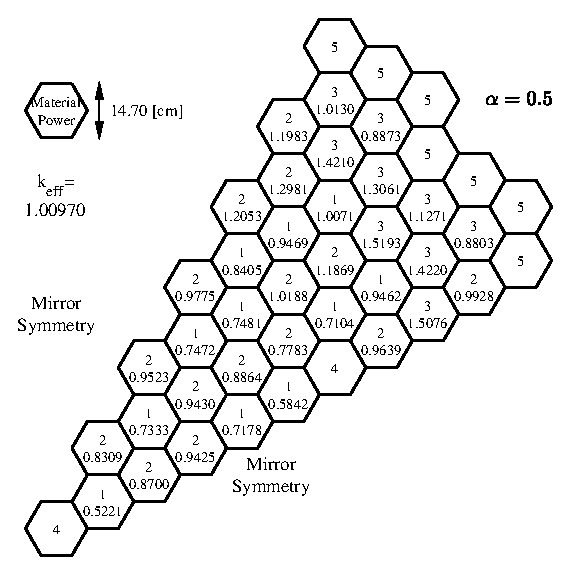
\includegraphics[width=0.7\textwidth]{vver440}
      \caption{VVER440 Geometry.}
      \label{fig:vver440_geom}
    \end{figure}

    \begin{table}
      \caption{VVER440 Cross Sections.}
      \label{tab:vver440xs}
      \begin{center}
        \begin{tabular}{cccccc}
          \toprule
          &MAT1&MAT2&MAT3&MAT4&MAT5\\
          \midrule
          $D_1$&1.346600E+00&1.337700E+00&1.332200E+00&1.195300E+00&1.448500E+00\\
          $D_2$&3.716900E-01&3.691800E-01&3.650200E-01&1.931300E-01&2.517600E-01\\
          $\Sigma_{r1}$&2.525500E-02&2.470900E-02&2.435000E-02&3.563600E-02&3.318400E-02\\
          $\Sigma_{r2}$&6.427700E-02&7.936100E-02&1.001000E-01&1.349800E-01&3.283900E-02\\
          $\Sigma_{s 1\rightarrow 2}$&1.689300E-02&1.591200E-02&1.488800E-02&2.226400E-02&3.226200E-02\\
          $ \nu \Sigma_{f1}$&4.448800E-03&5.533700E-03&7.039100E-03&&\\
          $ \nu \Sigma_{f2}$&7.375300E-02&1.058100E-01&1.496400E-01&&\\
          \bottomrule
        \end{tabular}
      \end{center}
    \end{table}

    \begin{table}
      \caption{VVER440 Fission Spectrum.}
      \label{tab:vver440chi}
      \begin{center}
        \begin{tabular}{cc}
          \toprule
          &Fission Spectrum \\
          \midrule
          $\chi_1$ & 1.00000E+00  \\
          $\chi_2$ & 0.00000E+00  \\
          \bottomrule
        \end{tabular}
      \end{center}
    \end{table}

  \subsection{SNR}
    \label{sec:snr}
    This benchmark is presented with solution in the Argonne Code Center
    Benchmark Problem Book \cite{argonneBenchmark}. It
    is based on the MARK-I core design of the SNR-300. The problem is
    one-twelfth of a reactor with no control rods inserted. There are 17
    assemblies across the core diameter with the outer rings being blanket
    assemblies as shown in \fref{fig:snr_geom}. Each assembly has a flat-to-flat
    measurement of 11.20 \units{cm}. Vacuum boundary condition ($\albedo =
    0.5$) is applied on the core periphery and all other boundaries are mirror
    boundary conditions ($\grad \phi \cdot \nhat = 0$). To the precision of the 
    benchmark, the effective neutron multiplication factor is $\keff = 1.124$. 
    Assembly powers are not provided in the benchmark but can be calculated from 
    existing codes (e.g. \dif).

    \begin{figure}
      \centering
      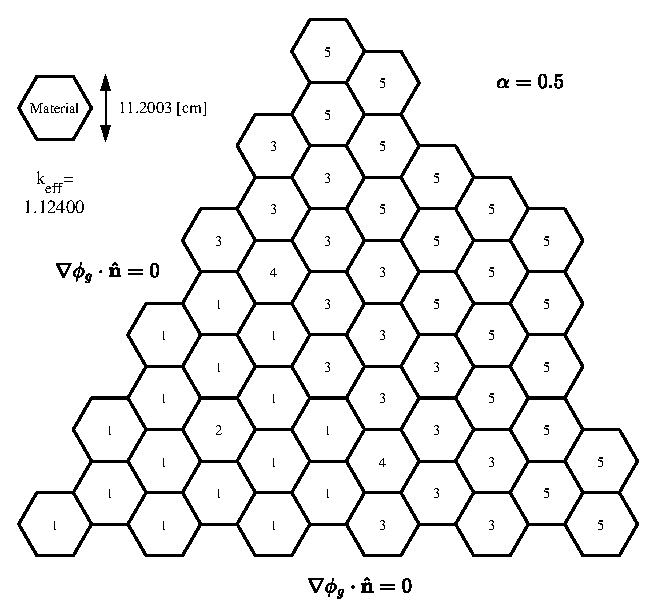
\includegraphics[width=0.7\textwidth]{snr}
      \caption{SNR Geometry.}
      \label{fig:snr_geom}
    \end{figure}

    \newgeometry{margin=1in,lmargin=1.25in,footskip=\chapterfootskip, includehead, includefoot}
    \thispagestyle{lscapedplain}
    \begin{landscape}
    \begin{table}
      \caption{SNR Cross Sections.}
      \label{tab:snrxs}
      \begin{center}
        \begin{tabular}{ccccccc}
          \toprule
          &MAT1&MAT2&MAT3&MAT4&MAT5&MAT6\\
          \midrule
          $D_1$&2.876787E+00&2.876539E+00&2.285610E+00&2.716653E+00&2.503066E+00&4.616422E+00\\
          $D_2$&1.570845E+00&1.571363E+00&1.171935E+00&1.440943E+00&1.314665E+00&2.901831E+00\\
          $D_3$&7.224859E-01&7.127076E-01&6.324751E-01&7.203469E-01&5.742770E-01&1.021179E+00\\
          $D_4$&9.641993E-01&9.429781E-01&8.183574E-01&9.876836E-01&6.153695E-01&1.729625E+00\\
          $\Sigma_{r1}$&2.820400E-02&2.878200E-02&3.595900E-02&2.909300E-02&2.481400E-02&1.315900E-02\\
          $\Sigma_{r2}$&5.274700E-03&6.049100E-03&5.885500E-03&4.490900E-03&1.641200E-02&1.455900E-03\\
          $\Sigma_{r3}$&1.761200E-02&1.951000E-02&1.604100E-02&1.308200E-02&7.212200E-02&4.600100E-03\\
          $\Sigma_{r4}$&2.654600E-02&3.371400E-02&1.334900E-02&9.956200E-03&1.686800E-01&7.866000E-04\\
          $\Sigma_{s 1\rightarrow 2}$&2.359700E-02&2.326200E-02&3.207100E-02&2.632200E-02&2.294600E-02&1.294200E-02\\
          $\Sigma_{s 1\rightarrow 3}$&4.079100E-06&4.645100E-06&3.888000E-06&2.890700E-06&1.032000E-06&6.878000E-07\\
          $\Sigma_{s 2\rightarrow 3}$&1.615300E-03&1.571800E-03&2.777600E-03&2.288900E-03&3.768700E-03&1.287100E-03\\
          $\Sigma_{s 1\rightarrow 4}$&4.449300E-08&4.996800E-08&4.503900E-08&3.324800E-08&1.048900E-08&6.990300E-09\\
          $\Sigma_{s 2\rightarrow 4}$&4.230900E-08&4.072400E-08&9.001800E-08&6.213300E-08&7.036100E-12&4.363300E-12\\
          $\Sigma_{s 3\rightarrow 4}$&4.683800E-03&4.341400E-03&5.897100E-03&5.353600E-03&8.681500E-03&3.453300E-03\\
          $ \nu \Sigma_{f1}$&1.187800E-02&1.494300E-02&7.742700E-03&5.427900E-03&&\\
          $ \nu \Sigma_{f2}$&5.325200E-03&7.688700E-03&1.082500E-04&7.585700E-05&&\\
          $ \nu \Sigma_{f3}$&1.047100E-02&1.480900E-02&2.974200E-04&2.121799E-04&&\\
          $ \nu \Sigma_{f4}$&2.661100E-02&3.815900E-02&8.468699E-04&5.759200E-04&&\\
          \bottomrule
        \end{tabular}
      \end{center}
    \end{table}
    \end{landscape}
    \restoregeometry
    \pagestyle{plain}
    \thispagestyle{plain}
    \newgeometry{margin=1in,lmargin=1.25in,footskip=\chapterfootskip, includehead, includefoot}

    \begin{table}
      \caption{SNR Fission Spectrum.}
      \label{tab:snrchi}
      \begin{center}
        \begin{tabular}{cc}
          \toprule
          &Fission Spectrum \\
          \midrule
          $\chi_1$ &0.768 \\
          $\chi_2$ &0.232 \\
          $\chi_3$ &0.000 \\
          $\chi_4$ &0.000 \\
          \bottomrule
        \end{tabular}
      \end{center}
    \end{table}

  \subsection{\texorpdfstring{\glsentryshort{hwr}}{HWR}}
    \label{sec:hwr}
    This benchmark is presented with solution by Chao and Shatilla \cite{chao}. 
    It is based on a
    very large \gls{hwr}. The problem is one-sixth rotationally symmetric 
    (\textit{not} reflective). For code packages without rotational boundary 
    conditions, it will be necessary to simulate a full core. The problem is 
    large with 35 assemblies across the core diameter as shown in 
    \fref{fig:hwr_geom}. Each assembly has a flat-to-flat measurement of 17.78
    \units{cm}. The fueled assemblies are surrounded by a tritium 
    generating zone which is then surrounded by a reflector zone. Zero-flux 
    boundary condition ($\phi = 0$) is applied on the core periphery. This is 
    the only benchmark with such a boundary condition. Cross sections are 
    provided in \tref{tab:hwrxs}. The fission spectrum is specified in 
    \tref{tab:hwrchi}. To the precision of the benchmark, the effective neutron 
    multiplication factor is $\keff = 0.991965$. Assembly powers are given in 
    \fref{fig:hwr_geom}.

    \begin{figure}
      \centering
      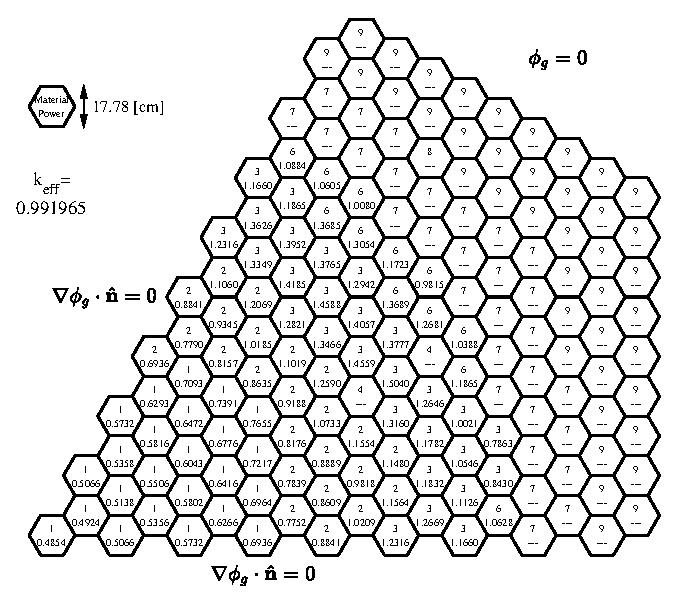
\includegraphics[width=\textwidth]{hwr}
      \caption{\glsentryshort{hwr} Geometry.}
      \label{fig:hwr_geom}
    \end{figure}

    \begin{table}
      \caption{\glsentryshort{hwr} Cross Sections.}
      \label{tab:hwrxs}
      \begin{center}
        \begin{tabular}{cccccc}
          \toprule
          &MAT1&MAT2&MAT3&MAT4&MAT5\\
          \midrule
          $D_1$&1.382500E+00&1.382550E+00&1.374420E+00&1.311980E+00&1.200000E+00\\
          $D_2$&8.975220E-01&8.974900E-01&8.883680E-01&8.799140E-01&9.000010E-01\\
          $\Sigma_{r1}$&1.110580E-02&1.117460E-02&1.062040E-02&1.268800E-02&1.268800E-02\\
          $\Sigma_{r2}$&2.230650E-02&2.238760E-02&1.694650E-02&5.290090E-04&5.300000E-04\\
          $\Sigma_{s 1\rightarrow 2}$&8.164570E-03&8.223780E-03&8.088160E-03&1.231150E-02&1.231150E-02\\
          $ \nu \Sigma_{f1}$&2.262160E-03&2.227500E-03&2.142810E-03&&\\
          $ \nu \Sigma_{f2}$&2.306230E-02&2.268490E-02&2.048870E-02&&\\
          \midrule
          &MAT6&MAT7&MAT8&MAT9&\\
          \midrule
          $D_1$&1.381390E+00&1.305990E+00&1.291930E+00&1.065100E+00&\\
          $D_2$&9.036710E-01&8.372560E-01&8.193410E-01&3.228290E-01&\\
          $\Sigma_{r1}$&1.056310E-02&1.173130E-02&1.191530E-02&2.834620E-02&\\
          $\Sigma_{r2}$&2.190300E-02&4.333040E-03&3.005650E-04&3.334890E-02&\\
          $\Sigma_{s 1\rightarrow
          2}$&7.765680E-03&1.109750E-02&1.155820E-02&2.619800E-02&\\
          $ \nu \Sigma_{f1}$&2.394690E-03&&&&\\
          $ \nu \Sigma_{f2}$&2.662100E-02&&&&\\
          \bottomrule
        \end{tabular}
      \end{center}
    \end{table}

    \begin{table}
      \caption{\glsentryshort{hwr} Fission Spectrum.}
      \label{tab:hwrchi}
      \begin{center}
        \begin{tabular}{cc}
          \toprule
          &Fission Spectrum \\
          \midrule
          $\chi_1$&1.00000E+00  \\
          $\chi_2$&0.00000E+00  \\
          \bottomrule
        \end{tabular}
      \end{center}
    \end{table}

  \subsection{IAEA}
    \label{sec:iaea}
    The IAEA \gls{pwr} problem was originally proposed for square lattice
    \glspl{pwr} but has been modified for a hexagonal geometry. This 
    modification is presented with solution by Chao and Shatilla \cite{chao}. 
    The problem is one-twelfth of a 
    reactor core. This problem has a total of four cases, with and without a 
    reflector ring added to the external core and with the albedo condition set 
    to $\albedo = 0.5$ and $\albedo = 0.125$. Each assembly has a flat-to-flat
    measurement of 20.0 \units{cm}. In the unreflected case, there are seven
    15 assemblies across the core diameter. In the reflected case, there are 16
    assemblies across the core diameter. To the precision of the benchmark, the
    effective neutron multiplication factors for each of the four cases is 
    summarized in \tref{tab:iaeakeff}.
    Assembly geometry and powers is provided for without and with 
    reflector in \fref{fig:iaea_geom}. All cross sections are provided in 
    \tref{tab:iaeaxs}. Fission spectrum is provided in \tref{tab:iaeachi}.

    \begin{table}
      \caption{IAEA Effective Neutron Multiplication Factors.}
      \label{tab:iaeakeff}
      \begin{center}
        \begin{tabular}{llc}
          \toprule
          Reflector & albedo ($\albedo$) & $\keff$ \\
          \midrule
          Without & 0.125 & 0.991378 \\
          Without & 0.5   & 0.978077 \\
          With    & 0.125 & 1.006630 \\
          With    & 0.5   & 1.005507 \\
          \bottomrule
        \end{tabular}
      \end{center}
    \end{table}

    \begin{figure}
      \centering
      \subfloat[Unreflected IAEA.]
        {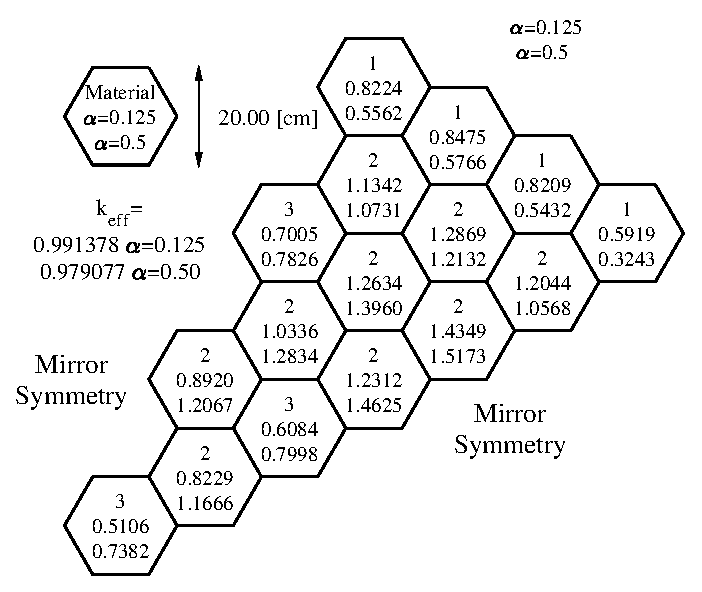
\includegraphics[width=0.7\textwidth]{iaea_nore}}
      \vspace{0.2in}
      \subfloat[Reflected IAEA.]
        {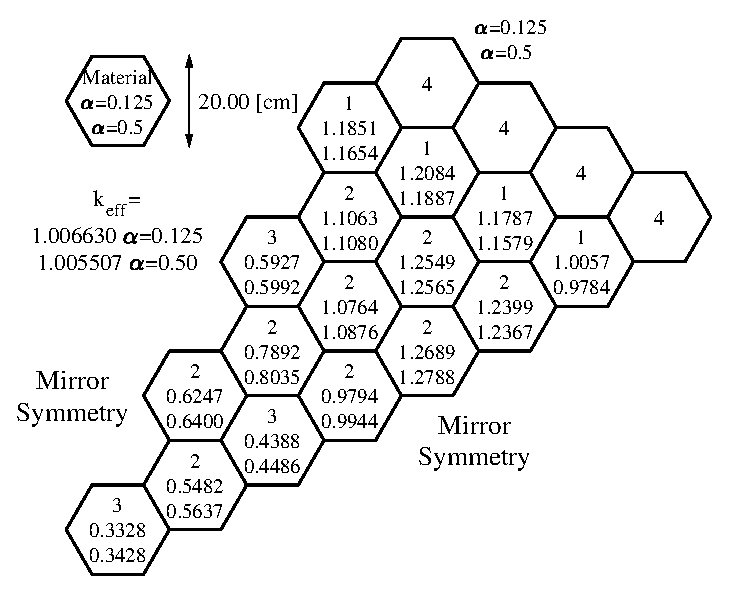
\includegraphics[width=0.7\textwidth]{iaea_refl}}
      \caption{IAEA Reflector Geometry.}
      \label{fig:iaea_geom}
    \end{figure}

    \begin{table}
      \caption{IAEA Cross Sections.}
      \label{tab:iaeaxs}
      \begin{center}
        \begin{tabular}{ccccc}
          \toprule
          &MAT1&MAT2&MAT3&MAT4\\
          \midrule
          $D_1$&1.500001E+00&1.500000E+00&1.500001E+00&1.500000E+00\\
          $D_2$&4.000001E-01&4.000000E-01&4.000001E-01&4.000000E-01\\
          $\Sigma_{r1}$&3.000000E-02&3.000000E-02&3.000000E-02&4.000000E-02\\
          $\Sigma_{r2}$&8.000000E-02&8.500000E-02&1.300000E-01&1.000000E-02\\
          $\Sigma_{s 1\rightarrow 2}$&2.000000E-02&2.000000E-02&2.000000E-02&4.000000E-02\\
          $ \nu \Sigma_{f1}$&0.000000E+00&0.000000E+00&0.000000E+00&\\
          $ \nu \Sigma_{f2}$&1.350000E-01&1.350000E-01&1.350000E-01&\\
          \bottomrule
        \end{tabular}
      \end{center}
    \end{table}

    \begin{table}
      \caption{IAEA Fission Spectrum.}
      \label{tab:iaeachi}
      \begin{center}
        \begin{tabular}{cc}
          \toprule
          &Fission Spectrum \\
          \midrule
          $\chi_1$&1.00000E+00  \\
          $\chi_1$&0.00000E+00  \\
          \bottomrule
        \end{tabular}
      \end{center}
    \end{table}

\section{Three-Dimension}
  For three-dimensional benchmarks, control rod worth
  measurement is instead used to observe agreement of the diffusion solution 
  to the benchmark solution. To measure control rod worth, three cases are run
  $\{A,B,C\}$ with control rods fully removed in case $A$, partially inserted
  in case $B$, and fully inserted in case $C$. 
  Rod worth is presented in 
  units \units{$\Delta k$} and calculated as 
  \begin{equation}
    \text{Rod Worth}_x \units{$\Delta k$} = \frac{\keffsub{A} - \keffsub{x}}
      {\keffsub{A} \, \keffsub{x}}
  \end{equation}
  for $x = \{B,C\}$. That is, rod worth is always compared to the case with
  control rods fully removed, case $A$. Additionally, Rod Difference is
  presented in units \units{$\% \Delta$k} as
  \begin{equation}
    \text{Rod Difference}_x \units{$\% \Delta k$} = (\keffsub{A} - \keffsub{x}) 
      \times 100 \%
  \end{equation}
  for $x = \{B,C\}$.

  \subsection{MONJU}
    \label{sec:monju}
    This benchmark is presented with solution by Komano et al. 
    \cite{monjuBenchmark}. It is
    based on a prototype \gls{fbr} with hexagonal pitch. The reactor
    has one-third rotational (\textit{not} reflective) symmetry. For code
    packages without rotational boundary conditions, it will be necessary to
    simulate a full core. There are 21 assemblies across the core diameter with
    outer rings being blanket assemblies as shown in \fref{fig:monju_geom}.
    Each assembly has a flat-to-flat measurement of 11.56 \units{cm}. Vacuum
    boundary condition ($\albedo = 0.5$) is applied on the core periphery. Cross
    sections are provided in \tref{tab:monjuxs}. No fission spectrum is
    specified in the benchmark but the one used in these simulations is provided
    in \tref{tab:monjuchi}. In determining this fission spectrum, it was
    observed that the benchmark results are not highly sensitive to the fission 
    spectrum.

    The reactor is simulated with three different control rod configurations; 
    patterns A, B, and C. Axially, all problems have a lower blanket extending
    from 0 \units{cm} to 30 \units{cm} and an upper blanket extending from
    121.5 \units{cm} to 151.5 \units{cm}. Fuel (in fueled assemblies) extends
    from 30 \units{cm} to 121.5 \units{cm}. In blanket assemblies, all material
    is blanket. The axial geometry of assemblies is shown in
    \fref{fig:monju_assy_geom}.

    In pattern A, all control rods are withdrawn and channels are simulated with
    sodium in the channel for the extend of the problem (0 \units{cm} to 151.5
    \units{cm}). In pattern B, control rods in rings 5 and 6 (per the numbering
    in \fref{fig:monju_geom}) are half way
    inserted and all others remain withdrawn. Control material occupies 
    75.75 \units{cm} to 151.5 \units{cm} and sodium material occupies 
    0 \units{cm} to 75.5 \units{cm}. In pattern C, the control assemblies in
    ring 5 and 6 that were previously half inserted are fully inserted and
    occupy 0 \units{cm} to 151.5~\units{cm}. Control rod withdrawal patterns are
    shown in \fref{fig:monju_cr_geom}. 
    
    Reference effective neutron
    multiplication factors and control rod worths are provided in
    \tref{tab:monjukeff}.

    \begin{table}
      \caption{MONJU Effective Neutron Multiplication Factors and Rod Worths.}
      \label{tab:monjukeff}
      \begin{center}
        \begin{tabular}{cccc}
          \toprule
          Pattern & $\keff$ & Rod Worth \units{$\Delta k$} & Rod Difference
            \units{$\% \Delta k$} \\
          \midrule
          A & 1.0723 &       & \\
          B & 1.0464 & 0.023 & 2.59 \\
          C & 1.0224 & 0.046 & 4.99 \\
          \bottomrule
        \end{tabular}
      \end{center}
    \end{table}

    \begin{figure}
      \centering
      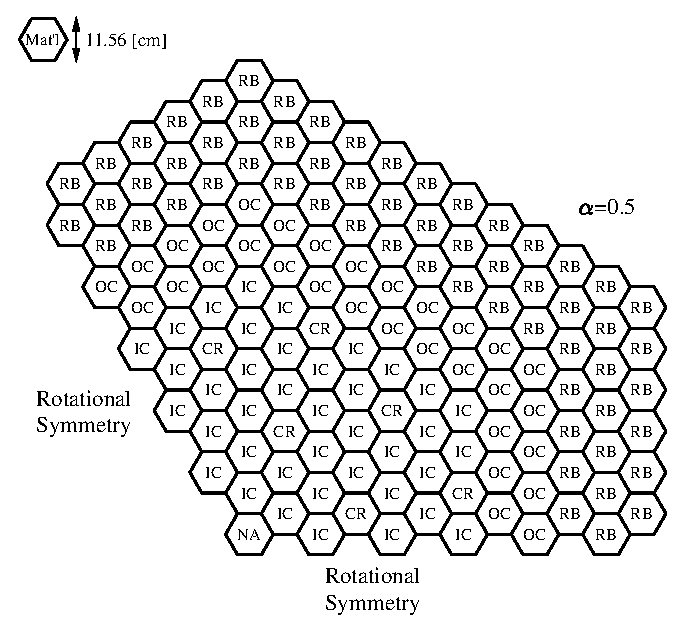
\includegraphics[width=0.7\textwidth]{monju}
      \caption{MONJU Geometry.}
      \label{fig:monju_geom}
    \end{figure}

    \begin{figure}
      \centering
      \subfloat[Assembly Geometry.]{
        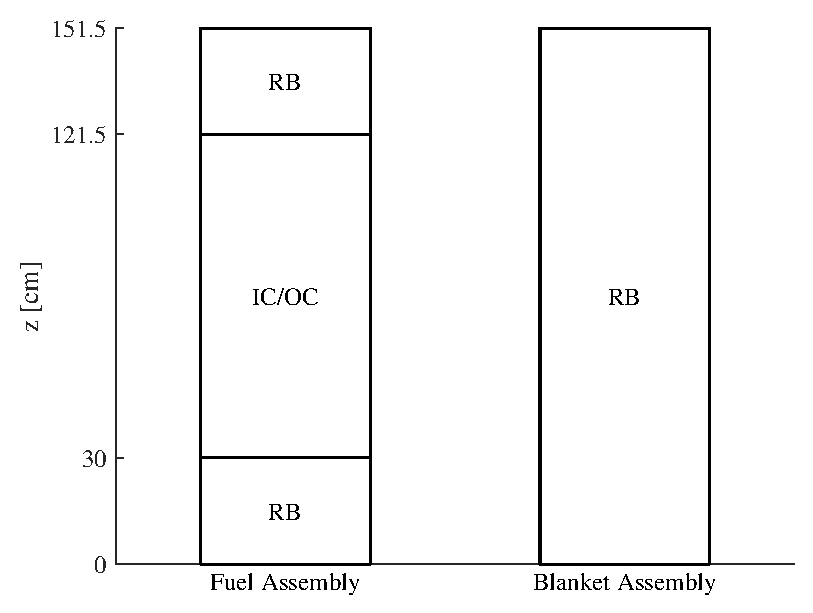
\includegraphics[width=0.45\textwidth]{monju_assembly_geometry}
        \label{fig:monju_assy_geom}}
      \hfill
      \subfloat[Control Rod Geometry.]{
        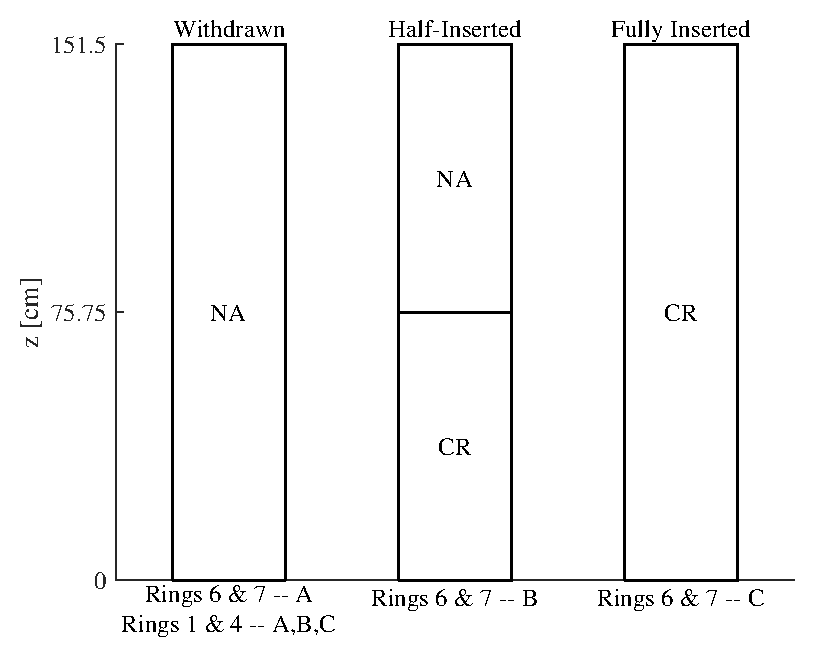
\includegraphics[width=0.45\textwidth]{monju_control_rod_geometry}
        \label{fig:monju_cr_geom}}
      \caption{MONJU Assembly Geometries.}
    \end{figure}

    \begin{table}
      \caption{MONJU Cross Sections.}
      \label{tab:monjuxs}
      \begin{center}
        \begin{tabular}{cccccc}
          \toprule
          &IC&OC&RB&CR&NA\\
          \midrule
          $D_1$&2.540000E+00&2.547990E+00&2.173000E+00&2.500010E+00&4.805000E+00\\
          $D_2$&1.724000E+00&1.725000E+00&1.439000E+00&1.681000E+00&3.262000E+00\\
          $D_3$&1.264000E+00&1.269000E+00&1.026000E+00&1.269000E+00&2.431000E+00\\
          $\Sigma_{r1}$&3.098650E-02&3.121380E-02&3.793080E-02&2.328030E-02&1.152508E-02\\
          $\Sigma_{r2}$&9.490000E-03&9.875000E-03&1.184300E-02&1.272700E-02&3.648740E-03\\
          $\Sigma_{r3}$&7.333000E-03&8.099000E-03&7.611000E-03&1.497000E-02&3.072000E-04\\
          $\Sigma_{s 1\rightarrow 2}$&2.544000E-02&2.497000E-02&3.288000E-02&2.185000E-02&1.130000E-02\\
          $\Sigma_{s 1\rightarrow 3}$&5.625000E-04&5.548000E-04&7.468000E-04&2.163000E-04&6.718000E-05\\
          $\Sigma_{s 2\rightarrow 3}$&6.551000E-03&6.341000E-03&1.000000E-02&9.379000E-03&3.571000E-03\\
          $ \nu \Sigma_{f1}$&1.235000E-02&1.467000E-02&8.631000E-03&&\\
          $ \nu \Sigma_{f2}$&5.225000E-03&6.955000E-03&5.995000E-04&&\\
          $ \nu \Sigma_{f3}$&7.684000E-03&9.986000E-03&1.381000E-03&&\\
          \bottomrule
        \end{tabular}
      \end{center}
    \end{table}

    \begin{table}
      \caption{MONJU Fission Spectrum.}
      \label{tab:monjuchi}
      \begin{center}
        \begin{tabular}{cc}
          \toprule
          &Fission Spectrum \\
          \midrule
          $\chi_1$&7.81200E-01  \\
          $\chi_2$&2.09940E-01  \\
          $\chi_3$&8.86000E-03  \\
          \bottomrule
        \end{tabular}
      \end{center}
    \end{table}

  \subsection{KNK}
    \label{sec:knk}
    This benchmark is presented with solution by Takeda and Ikeda 
    \cite{takedaBenchmark}. It is
    based on a small \gls{fbr} with hexagonal-$z$ geometry and is
    a model of the KNK-II core. The reactor has one-third rotational
    (\textit{not} reflective) symmetry. For code packages without rotational
    boundary conditions, it will be necessary to simulate a full core. There are
    15 assemblies across the core diameter with outer rings of reflectors and
    steel as shown in \fref{fig:knk_geom}. Each assembly has a flat-to-flat
    measurement of 12.99 \units{cm}. Vacuum boundary condition ($\albedo = 0.5$)
    is applied on the core periphery. Cross sections are provided in
    \tref{tab:knkxs_a} and \tref{tab:knkxs_b}. The fission spectrum is provided
    in \tref{tab:knkchi}.

    The reactor is simulated with three different control rod configurations;
    patterns A, B, and C. In pattern A, all control rods are withdrawn. In
    pattern B, control rods are half inserted into the active fuel region. In
    pattern C, control rods are fully inserted into the active fuel region. All
    axial geometries are shown in \fref{fig:knk_cr_geom}. The axial geometry
    for control rod withdrawal is shown in \fref{fig:knk_cr_geom}.
    Reference effective neutron multiplication factors and control rod worths 
    are provided in \tref{tab:knkkeff}.

    Reference results for the KNK problem are presented for the solution to the
    neutron transport equation. The reference presents Monte Carlo solutions and
    other solutions to the neutron transport equation and these converge to
    the same solution. For diffusion solutions to these simulations, agreement
    is expected to within some tolerance. However, comparison can also be
    difficult as the equations solved are entirely different.

    \begin{table}
      \caption{KNK Effective Neutron Multiplication Factors and Rod Worths.}
      \label{tab:knkkeff}
      \begin{center}
        \begin{tabular}{cccc}
          \toprule
          Pattern & $\keff$ & Rod Worth \units{$\Delta k$} & Rod Difference
            \units{$\% \Delta k$} \\
          \midrule
          A & 1.0951 &       & \\
          B & 1.9833 & 0.104 & 11.18 \\
          C & 0.8799 & 0.223 & 21.52 \\
          \bottomrule
        \end{tabular}
      \end{center}
    \end{table}

    \begin{figure}
      \centering
      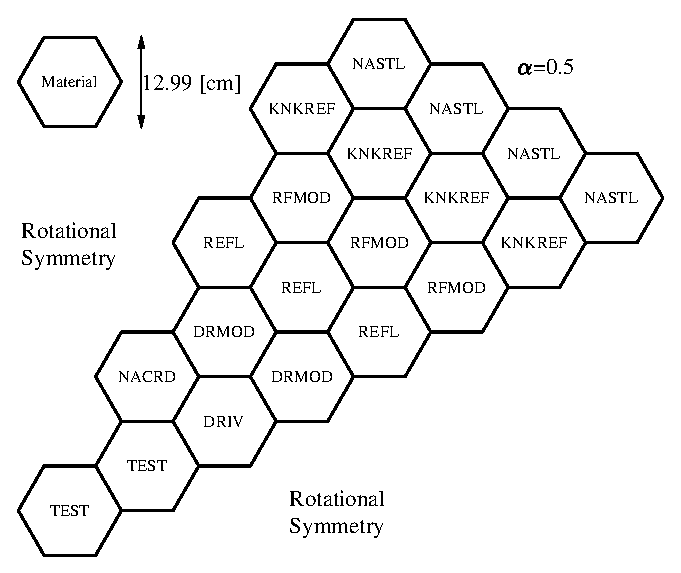
\includegraphics[width=0.7\textwidth]{knk}
      \caption{KNK Geometry.}
      \label{fig:knk_geom}
    \end{figure}

    \begin{figure}
      \centering
      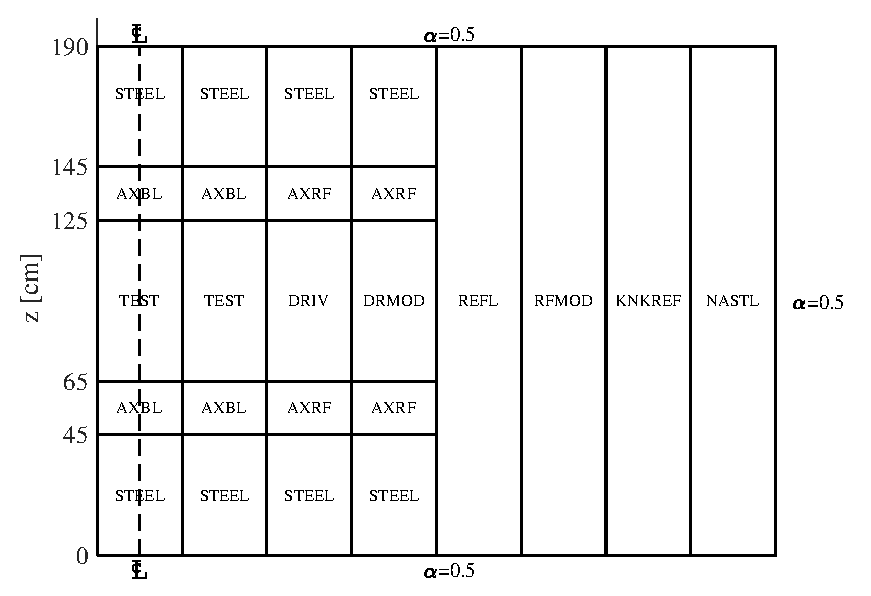
\includegraphics[width=0.7\textwidth]{knk_assembly_geometry}
      \caption{KNK Assembly Geometry.}
      \label{fig:knk_assembly_geom}
    \end{figure}

    \begin{figure}
      \centering
      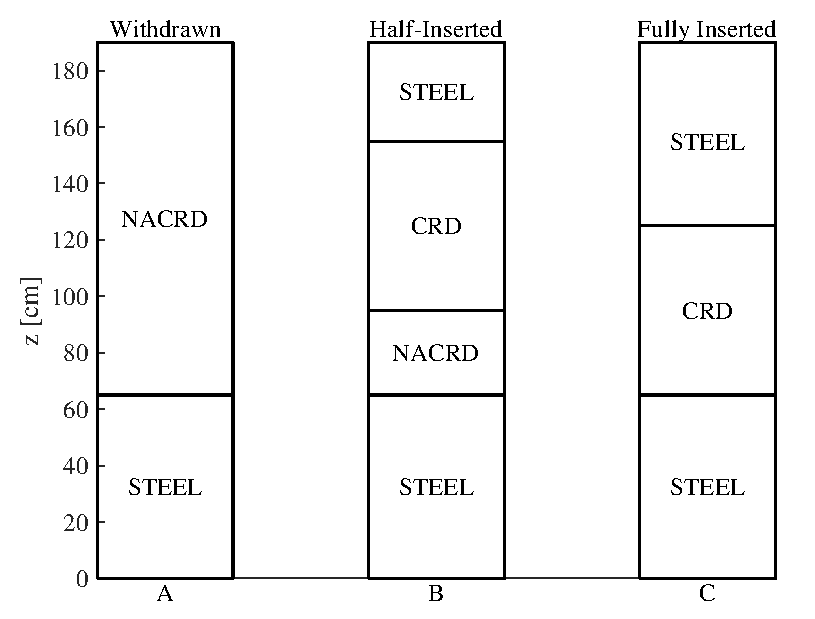
\includegraphics[width=0.7\textwidth]{knk_control_rod_geometry}
      \caption{KNK Control Rod Geometry.}
      \label{fig:knk_cr_geom}
    \end{figure}
    
    \newgeometry{margin=1in,lmargin=1.25in,footskip=\chapterfootskip, includehead, includefoot}
    \thispagestyle{lscapedplain}
    \begin{landscape}
    \begin{table}
      \caption{KNK Cross Sections (Part A).}
      \label{tab:knkxs_a}
      \begin{center}
        \begin{tabular}{cccccccc}
          \toprule
          &STEEL&AXBL&AXRF&TEST&DRIV&DRMOD&REFL\\
          \midrule
          $D_1$&3.388781E+00&2.373121E+00&2.507529E+00&2.676817E+00&2.377115E+00&2.356912E+00&2.091884E+00\\
          $D_2$&2.466578E+00&1.477974E+00&1.867089E+00&1.658169E+00&1.460419E+00&1.358360E+00&1.540678E+00\\
          $D_3$&1.483136E+00&1.019165E+00&1.177228E+00&1.163065E+00&1.023104E+00&8.369847E-01&9.559535E-01\\
          $D_4$&1.177370E+00&9.768754E-01&7.212400E-01&9.039009E-01&7.968248E-01&7.645435E-01&5.339750E-01\\
          $\Sigma_{r1}$&7.758804E-03&1.665700E-02&9.938010E-03&1.856200E-02&2.033901E-02&2.709099E-02&1.137701E-02\\
          $\Sigma_{r2}$&4.558990E-03&8.274010E-03&5.436010E-03&1.165498E-02&1.303201E-02&3.338801E-02&5.945000E-03\\
          $\Sigma_{r3}$&5.202000E-03&9.116980E-03&5.957010E-03&1.639202E-02&1.892099E-02&4.616198E-02&6.607000E-03\\
          $\Sigma_{r4}$&2.410000E-03&9.943000E-03&3.569000E-03&4.981199E-02&5.742100E-02&6.511802E-02&4.942950E-03\\
          $\Sigma_{s 1\rightarrow 1}$&9.060500E-02&1.238050E-01&1.229950E-01&1.059640E-01&1.198870E-01&1.143370E-01&1.479690E-01\\
          $\Sigma_{s 1\rightarrow 2}$&7.423770E-03&1.454830E-02&9.412310E-03&1.127380E-02&1.307900E-02&2.096640E-02&1.066070E-02\\
          $\Sigma_{s 2\rightarrow 2}$&1.305810E-01&2.172600E-01&1.730950E-01&1.893700E-01&2.152130E-01&2.120060E-01&2.104100E-01\\
          $\Sigma_{s 1\rightarrow 3}$&1.181630E-04&1.702760E-04&1.937910E-04&1.461920E-04&1.599380E-04&1.391320E-03&2.499560E-04\\
          $\Sigma_{s 2\rightarrow 3}$&4.352500E-03&6.788850E-03&5.098810E-03&3.648470E-03&4.001170E-03&2.672690E-02&5.467110E-03\\
          $\Sigma_{s 3\rightarrow 3}$&2.195470E-01&3.179480E-01&2.771940E-01&2.702070E-01&3.068850E-01&3.520930E-01&3.420850E-01\\
          $\Sigma_{s 1\rightarrow 4}$&8.258900E-07&9.370830E-07&1.393070E-06&9.621780E-07&1.071660E-06&6.102810E-05&1.825650E-06\\
          $\Sigma_{s 2\rightarrow 4}$&3.416750E-07&6.047930E-06&7.050750E-07&1.068880E-06&1.827160E-06&1.081860E-03&1.001570E-06\\
          $\Sigma_{s 3\rightarrow 4}$&4.645940E-03&4.387820E-03&5.096010E-03&1.804790E-03&1.673410E-03&3.290300E-02&5.368790E-03\\
          $\Sigma_{s 4\rightarrow 4}$&2.807070E-01&3.312810E-01&4.585980E-01&3.189600E-01&3.609060E-01&3.708720E-01&6.193060E-01\\
          $ \nu \Sigma_{f1}$&&2.961000E-03&&1.790430E-02&1.598780E-02&1.016630E-02&\\
          $ \nu \Sigma_{f2}$&&6.561700E-05&&1.599610E-02&1.644460E-02&9.463600E-03&\\
          $ \nu \Sigma_{f3}$&&1.146300E-04&&2.408560E-02&2.714500E-02&1.873250E-02&\\
          $ \nu \Sigma_{f4}$&&4.934825E-04&&7.331050E-02&8.458075E-02&8.253350E-02&\\
          \bottomrule
        \end{tabular}
      \end{center}
    \end{table}
    \end{landscape}
    \restoregeometry
    \pagestyle{plain}

    \newgeometry{margin=1in,lmargin=1.25in,footskip=\chapterfootskip, includehead, includefoot}
    \thispagestyle{lscapedplain}
    \begin{landscape}
    \begin{table}
      \caption{KNK Cross Sections (Part B).}
      \label{tab:knkxs_b}
      \begin{center}
        \begin{tabular}{cccccc}
          \toprule
          &RFMOD&KNKREF&NASTL&CRD&NACRD\\
          \midrule
          $D_1$&2.395256E+00&2.198131E+00&3.453884E+00&2.396616E+00&4.581354E+00\\
          $D_2$&1.349566E+00&2.341120E+00&3.376912E+00&1.461014E+00&3.326083E+00\\
          $D_3$&7.367704E-01&2.018587E+00&2.483855E+00&1.045568E+00&2.074220E+00\\
          $D_4$&6.215936E-01&4.141579E-01&8.077479E-01&5.313220E-01&2.199117E+00\\
          $\Sigma_{r1}$&3.325300E-02&1.321701E-02&8.154706E-03&2.136299E-02&6.395295E-03\\
          $\Sigma_{r2}$&6.217301E-02&4.880000E-03&3.460198E-03&3.345301E-02&4.094401E-03\\
          $\Sigma_{r3}$&7.935300E-02&4.410000E-03&3.444000E-03&7.445399E-02&4.686990E-03\\
          $\Sigma_{r4}$&2.415300E-02&5.912960E-03&3.037990E-03&3.125500E-01&1.207990E-03\\
          $\Sigma_{s 1\rightarrow 1}$&1.059110E-01&1.384270E-01&8.835500E-02&1.177220E-01&6.636340E-02\\
          $\Sigma_{s 1\rightarrow 2}$&2.964850E-02&1.239010E-02&7.734090E-03&1.260660E-02&6.233930E-03\\
          $\Sigma_{s 2\rightarrow 2}$&1.848200E-01&1.375020E-01&9.524930E-02&1.946990E-01&9.612360E-02\\
          $\Sigma_{s 1\rightarrow 3}$&3.065020E-03&3.669300E-04&1.947190E-04&1.333140E-04&7.021210E-05\\
          $\Sigma_{s 2\rightarrow 3}$&5.917800E-02&4.419270E-03&3.225680E-03&4.322190E-03&4.013750E-03\\
          $\Sigma_{s 3\rightarrow 3}$&3.730720E-01&1.607220E-01&1.307560E-01&2.443520E-01&1.560160E-01\\
          $\Sigma_{s 1\rightarrow 4}$&1.416970E-04&1.690360E-06&8.896150E-07&1.088390E-06&4.163880E-07\\
          $\Sigma_{s 2\rightarrow 4}$&2.692290E-03&1.632800E-06&7.984940E-07&1.854910E-07&1.269390E-07\\
          $\Sigma_{s 3\rightarrow 4}$&7.813260E-02&3.330750E-03&2.904810E-03&3.687810E-04&4.491110E-03\\
          $\Sigma_{s 4\rightarrow 4}$&5.121030E-01&7.989320E-01&4.096320E-01&3.148160E-01&1.503680E-01\\
          $ \nu \Sigma_{f1}$&&&&&\\
          $ \nu \Sigma_{f2}$&&&&&\\
          $ \nu \Sigma_{f3}$&&&&&\\
          $ \nu \Sigma_{f4}$&&&&&\\
          \bottomrule
        \end{tabular}
      \end{center}
    \end{table}
    \end{landscape}
    \restoregeometry
    \pagestyle{plain}
    \newgeometry{margin=1in,lmargin=1.25in,footskip=\chapterfootskip, includehead, includefoot}

    \begin{table}
      \caption{KNK Fission Spectrum.}
      \label{tab:knkchi}
      \begin{center}
        \begin{tabular}{cc}
          \toprule
          &Fission Spectrum \\ 
          \midrule
          $\chi_1$&0.908564 \\
          $\chi_2$&0.087307 \\
          $\chi_3$&0.004129 \\
          $\chi_4$&0.000000 \\
          \bottomrule
        \end{tabular}
      \end{center}
    \end{table}
